\documentclass{LabReport}
\title{操作系统实验报告PA4}
\author{221900180 田永铭}
\date{\today}
\addbibresource{refs.bib}
\Chead{操作系统实验报告PA4 221900180 田永铭}
\Cfoot{\thepage}
\usepackage{listings}
\usepackage{graphicx} 
\usepackage{tikzsymbols}
\usepackage{tikz}

\begin{document}
	\maketitle
	
	\tableofcontents
	
	\newpage
	
	\section{实验要求}
本次实验分为OS内核、API库、示范应用三个部分,为综合性实验项目(建议合理构造代码目录结构,采用makefile组织和管理整个实验项目的编译、部署和运行):\\
\begin{enumerate}
		\item 采用nasm汇编语言实现一个实验性质的OS内核并部署到MBR,主要功能如下:\\
1)实现write内核函数,向屏幕输出指定长度的字符串(尽量保证每次输出另起一行);\\
2)实现sleep内核函数,按整型参数以秒为单位延迟(以PA3为基础实现,包括设置定时器和时钟中断处理例程);\\
3)以系统调用的形式向外提供write和sleep两个系统服务(建议使用int 80h,也可分别以不同的用户自定义中断实现不同的系统服务,提供系统调用中断处理例程);\\
4)内核完成初始化后,从1号逻辑扇区开始加载示范性应用程序并运行(期间当应用进程sleep时,需切换至内核的无限循环处执行,当应用进程sleep结束时,需切换回应用进程执行)。
	\item 采用nasm汇编与C语言混合编程,实现一个API库\\
	1)提供一个包含write和sleep函数原型的C语言头文件(建议名称myos.h);\\
	2)用nasm汇编语言实现对应的API库(封装OS内核提供的两个系统调用服务,注意在此处妥善处理示范应用32位指令与OS内核16位指令的对接!!!)
	\item 采用C语言实现一个示范应用,并部署到磁盘\\
	1)采用C语言编写示范应用,用于测试OS内核功能,示范应用大致内容如下图所示(仅供参考!!!);\\
	2)采用GCC编译生成ELF32格式代码,并用objcopy等工具提取出相应的代码段和数据段,最后装入1号逻辑扇区开始的连续磁盘空间(由示范应用的大小确定)。\\
	提示:\\	
	1)MBR中的代码采用的是i8086体系架构上的16位指令(另需要注意代码尺寸,不能超越分区表!!!)\\	2)合理利用BIOS提供的基本输入输出功能:int10(屏幕输出),int 13(磁盘访问),int 16(键盘输入)\\
	
\end{enumerate}
	
	\section{实验环境}
	
	\begin{itemize}
		\item 操作系统:wsl2
		\item 编程语言:汇编语言 + C语言
		\item 使用工具:makefile;qemu;objdump;dd;nasm等
		\item 虚拟系统版本:windows-7;linux-20-desktop
	\end{itemize}
	
	\section{实验原理}
	\begin{itemize}
		\item \textbf{总体原理:} 在内核实现需要利用特权指令的功能,将其整理成接口暴露给上层的应用程序,应用程序通过调用接口,实现对内核函数的使用。
		
		\item \textbf{加载应用程序的原理:} 在计算机启动时,应用程序被加载并执行,部分原理已经在前几次作业完全搞清楚了,注意这次实验中要把应用程序加载到第一扇区。
		
		\item \textbf{write和sleep的原理:}write只需要调用BIOS功能int 10即可,相对简单。而sleep执行时,我的实现是:内核里面有一个idle进程(死循环),这个进程具有栈地址。在调用sleep的时候,cpu执行会先保存app下一条语句的栈地址,再从app的执行流程中,切换到idle进程执行,相当于是一次调度和切换。当sleep结束的时候,再从idle进程利用栈地址切换到app的进程中继续执行。
		
		\item \textbf{时钟中断原理:}已经在PA3中阐述清楚。
		
		\item \textbf{makefile的原理:}makefile 是一种用于构建和管理源代码的工具,它主要用于自动化软件编译过程。其原理基于一种称为``依赖关系"的概念,即文件之间的相互依赖关系。它通过这种依赖关系依次编译文件。
	\end{itemize}
	
	\section{实验结果展示}
	{\color{red} 注意:} 我的main函数是``写一个hello! \textbf{+} sleep一秒 \textbf{+}写一个goodbye! \textbf{+} sleep一秒”的循环。
	\begin{itemize}
		\item \textbf{视频展示: } \href{https://box.nju.edu.cn/f/a5787150680c45f38938/}{\color{red} 221900180\_田永铭\_实验4\_视频演示.mp4}
		\item \textbf{助教本地运行检验: } 只需要解压代码压缩文件,在wsl2环境下打开终端,只需运行``make"。如果没有配置好qemu路径,需要将qemu路径在代码对应位置填写完整。如果再运行不了,仍可通过利用wsl来make,再利用windows上的qemu来运行qemu下各个指令。本人确保已经能正常运行成功。
	\end{itemize}

	
	\section{最终成功的实验过程}
	
	{\color{red} 注意:} 此部分着重介绍最终成功的实验过程,而尝试过程、失败过程和各种debug过程见后面部分。\par
	\hspace{0em}实验主要分为以下几个步骤:
	
	\begin{enumerate}
		\item 配置环境
		\item 打通内核、调用接口、app,简单实现write
		\item 实现sleep
		\item 写入磁盘,查看运行效果
		\item 进行一些优化
	\end{enumerate}
	
	\subsection{配置环境}
由于wsl2环境下更利于本次实验makefile的使用,能够更好的链接好可执行文件,所以我首先配置了windows-11下的wsl2环境。\par
\hspace{0em}参考\href{https://blog.csdn.net/xiaouncle/article/details/136910057?utm_medium=distribute.pc_relevant.none-task-blog-2~default~baidujs_baidulandingword~default-0-136910057-blog-114636422.235^v43^pc_blog_bottom_relevance_base8&spm=1001.2101.3001.4242.1&utm_relevant_index=3}{\color{blue} wsl2的安装教程}, 首先安装好wsl2。再参考\href{https://blog.csdn.net/mmc02/article/details/136142015?ops_request_misc=%257B%2522request%255Fid%2522%253A%2522171377421816777224417656%2522%252C%2522scm%2522%253A%252220140713.130102334.pc%255Fall.%2522%257D&request_id=171377421816777224417656&biz_id=0&utm_medium=distribute.pc_search_result.none-task-blog-2~all~first_rank_ecpm_v1~rank_v31_ecpm-5-136142015-null-null.142^v100^pc_search_result_base5&utm_term=wsl2%E5%A6%82%E4%BD%95%E5%AF%BC%E5%85%A5vscode&spm=1018.2226.3001.4187}{\color{blue} vscode远程连接 wsl教程},配置vscode,添加WSL插件,在vscode中连接wsl环境。\par
\hspace{0em}工作区配置完成后,如下图所示,可以在vscode中方便地编写代码。
\begin{figure}[h!]
	\centering
	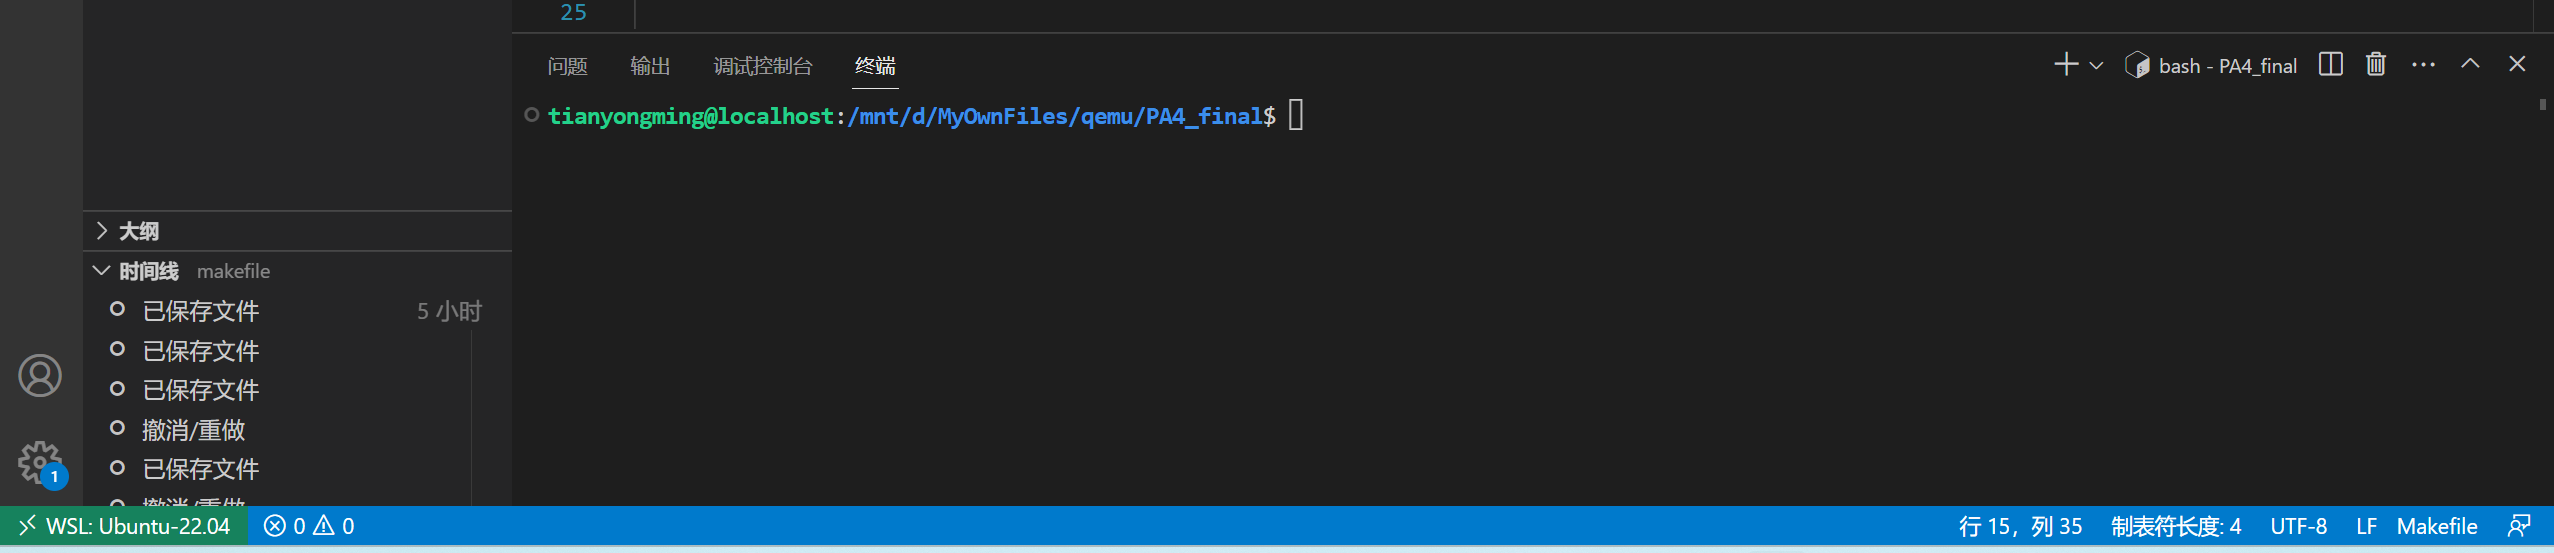
\includegraphics[width=0.7\linewidth]{C:/Users/86181/Desktop/figures/1}
	\caption{wsl2工作区}
	\label{fig:1}
\end{figure}

	\subsection{打通内核、调用接口、app,简单实现write}
	首先搭建起整套代码框架,打通内核、调用接口、app,简单实现write,这是比较关键的一步,实现了这一步,后面才调试得起来,才有写好sleep的可能。\\\\
	\subsubsection{确定代码框架}
	我使用了和助教一样的代码框架,框架如下(link.ld是我为了更好的链接而写的文件):\\\\\\\\\\\\

\begin{figure}[h!]
	\centering
	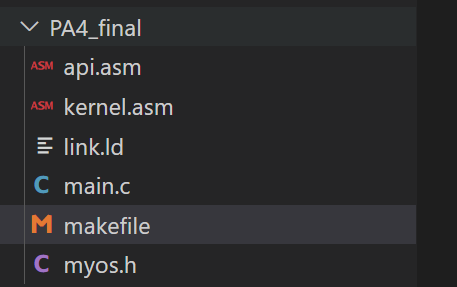
\includegraphics[width=0.7\linewidth]{C:/Users/86181/Desktop/figures/2}
	\caption{代码框架}
	\label{fig:2}
\end{figure}
	\subsubsection{编写myos.h和main.c}
	这部分最为简单,头文件定义函数的原型,上层应用文件就是简单的一直调用。针对我来说,我希望每次上层应用文件是``写一个hello! \textbf{+} sleep一秒 \textbf{+}写一个goodbye! \textbf{+} sleep一秒”的循环。代码如下:
	
	\begin{lstlisting}[language=python,frame=shadowbox]
; myos.h
#ifndef MYOS_H
#define MYOS_H

void write(char* str, int len);
void sleep(int seconds);

#endif
	\end{lstlisting}
	
	\begin{lstlisting}[language=python,frame=shadowbox]
; main.c
int main(void)
{   
	while(1)
	{
		write("hello!",6);
		sleep(1);
		write("goodbye!",8);
		sleep(1);
	}
}
	\end{lstlisting}
	
	\subsubsection{编写api}
	参考文献\href{https://blog.csdn.net/weixin_43216249/article/details/109827911}{\color{blue} 汇编实现过程体的调用教程}, 首先编写一个api暴露write的接口,通过esp来访问参数,同时注意保护栈以及32位下ret指令是retd。代码如下:
\begin{lstlisting}[language=python,frame=shadowbox]
BITS 16
section .text
global write
global sleep

write:
;保护栈
push ebp
mov  ebp, esp
push ebx
push ecx

mov  ebx, [ebp+8] ;地址
mov  ecx, [ebp+12] ;长度
int 0x80    ;调用中断

pop ecx
pop ebx
pop ebp
retd    ;回跳要用32位的指令,ret是16位的
\end{lstlisting}
参数是通过ebp来获取的,其中write有两个参数,需要两个寄存器来存储。然后再调用80号中断,来自动跳转到内核进行处理。
	
	\subsubsection{编写kernel}
仿照PA3,我们需要将80号用户自定义中断写入中断向量表,代码如下:
\begin{lstlisting}[language=python,frame=shadowbox]
mov word [0x80*4],write_handler
mov word [0x80*4+2],0
\end{lstlisting}
至于write\_handler的编写,可以先完全仿照PA3。仍有一部分关键的步骤是对app的加载,我们需要在内核函数运行结束之前,将其拉到第一扇区。根据老师所言,通过切换栈指针iret的方式来进行,我最终采用。代码如下:
\begin{lstlisting}[language=python,frame=shadowbox]
;加载应用程序
load_application:
xor ax,ax
mov es,ax 
mov bx,0x8000;  link.ld中定义text在0x8000
mov ah, 2    
mov al, 1      
mov ch, 0      
mov cl, 2          
mov dh, 0          
mov dl, 0x80    
int 0x13           
mov sp,0x8000 ;切换到应用栈
;   通过iret跳转应用进程执行
pushf
push word 0 ;cs
push word 0x8000; 
iret 
\end{lstlisting}
	\subsubsection{编写makefile}
	我在助教发makefile样例之前完成了对这个makefile的编写,中途出了非常多的问题,\textbf{这将在后一部分讨论},此处给出成功的实现和注释:
\begin{lstlisting}[language=python,frame=shadowbox]
# 运行命令: make即可
# 反汇编指令:objdump -D  -Mi8086,suffix app.elf
all:app.bin

app.bin:app.elf
objcopy -R.eh_frame \
-R \
.comment \
-O \
binary \
app.elf app.bin
make qemu

# 为了让被执行的第一个函数是main,用-e main
app.elf:main.o api.o 
ld -m \
elf_i386 \
-T link.ld \
-e main \
main.o api.o \
-o app.elf 

# 要用-m16
main.o:main.c myos.h
gcc -m16 \
-ffreestanding \
-fno-pic \
-I. \
-c main.c \
-o main.o

api.o:api.asm
nasm -f elf32 api.asm -o api.o

qemu:
qemu-img create -f raw PA4_disk.raw 5G
nasm -f bin -o kernel.bin kernel.asm
make dd

dd:
dd if=kernel.bin of=PA4_disk.raw bs=512 count=1
dd if=app.bin of=PA4_disk.raw bs=512 seek=1 count=1
# dd 命令中的 seek=1 用于将写入光标定位到磁盘映像文件(PA4_disk.raw)
# 的第1个扇区,然后再将来自 app.bin 的数据写入。
# 实现从第二个扇区开始写入 app.bin 的数据,而不是覆盖现有数据。
make run

run:
qemu-system-x86_64 -drive file=PA4_disk.raw,format=raw 
\end{lstlisting}

\textbf{至此,我已经完成了简单的write的打通。}在wsl2下运行make,发现能够非常迅速地打印hello!(此时我的应用程序还没写sleep)和goodbye!但是打印速度飞快,为了更好地看清,我先将main函数的while(1)改成了for循环语句,发现运行效果符合预期。

	\subsection{实现sleep}
	首先基于write的实现简单地模仿,更新api文件、main文件、myos头文件,在kernel文件中先将PA3中的时钟中断复用,再模仿write定义好sleep的81号中断。此部分代码很简单,略去不展示,详见附件中的代码。难点在于sleep时长的控制和进程的切换,实现如下:
	
	\subsubsection{sleep时长的控制}
	由于PA3中我的时钟中断是20ms一次,所以50次才是1s,所以需要注意参数的归一化。由api传来的秒数我存放在了ax中,我通过一个loop循环和几个段地址的计数器实现了sleep时长的控制,代码如下:
\begin{lstlisting}[language=python,frame=shadowbox]
clock_handler:
inc word [counter]; 增加一次counter的数值

mov dx, [num]
mov cx, [counter]
cmp cx, dx
;到点就跳转回去
je back_to_main
iret

loop:   ;归一化1s
mov dx, [normalize]
add ax, dx
dec cx
cmp cx, 0
je continue
jmp loop

sleep_handler:
cli
mov cx, 50  ;20ms*50=1s,cx存入50
mov [normalize], ax	;ax参数存入了normalize
jmp loop

continue:
mov [num], ax;loop后,次数ax已经是sleep需要的时钟中断的个数
sti ;一定要开中断,否则时钟中断被屏蔽,无法产生
\end{lstlisting}
	\subsubsection{进程的切换}
	\textbf{我最终是按照老师的要求,{\color{red} 全部}利用iret进行切换}。这有一个重要的理由:实际上OS都是有保护模式的,不能通过jmp在内核和应用程序间随意切换。\par
	\hspace{0em}简单来讲,当sleep开始时,调用了81号中断,操作系统从用户态陷入内核态,此时在内核态通过iret方式切换到idle进程,此后此idle进程会被时钟中断打断,统计到sleep时间达到后,需要切换栈指针,模仿iret的标准实现,从内核态安全地返回应用程序继续执行。核心代码如下:
\begin{lstlisting}[language=python,frame=shadowbox]
;此处是跳转idle的代码
;保护现场cx,dx
push cx
push dx
push bp
mov bp,sp;  bp此时就是回去的栈指针
mov sp,idle_stack ;切换到idle栈
;   通过iret跳转idle进程执行
pushf
push word 0 ;cs
push word idle; 
iret

;idle进程,除非要跳转回main函数,否则一直死循环
idle:
	jmp idle

;此处是返回main的代码
mov sp,bp  ;将堆栈指针设置为基址指针(Base Pointer,BP)的
	;实际上是将堆栈指针重新指向了应用程序的栈。
pop bp  ;弹出堆栈中的值,将其存入基址指针(BP)寄存器
	;这样恢复了应用程序的堆栈帧。
pop dx ;恢复现场
pop cx ;恢复现场
iret  ;通过iret回到app

\end{lstlisting}
	至此,我实现了sleep。当然这样的代码还会有问题,这将在后面讨论。
	
	\subsection{写入磁盘,查看运行效果}
	写入磁盘,运行效果符合预期。屏幕上间每隔1秒依次输出一个hello!或者goodbye!不过,此时我还没有换行,它们是连在一起输出的。这样的运行效果完全符合预期。
	
	\subsection{进行一些优化}
	\subsubsection{实现换行}
	为了实现换行,可以每次输出后打印一个换行,但是这会导致打印的东西错开,很丑,如下图所示:
\begin{figure}[h!]
	\centering
	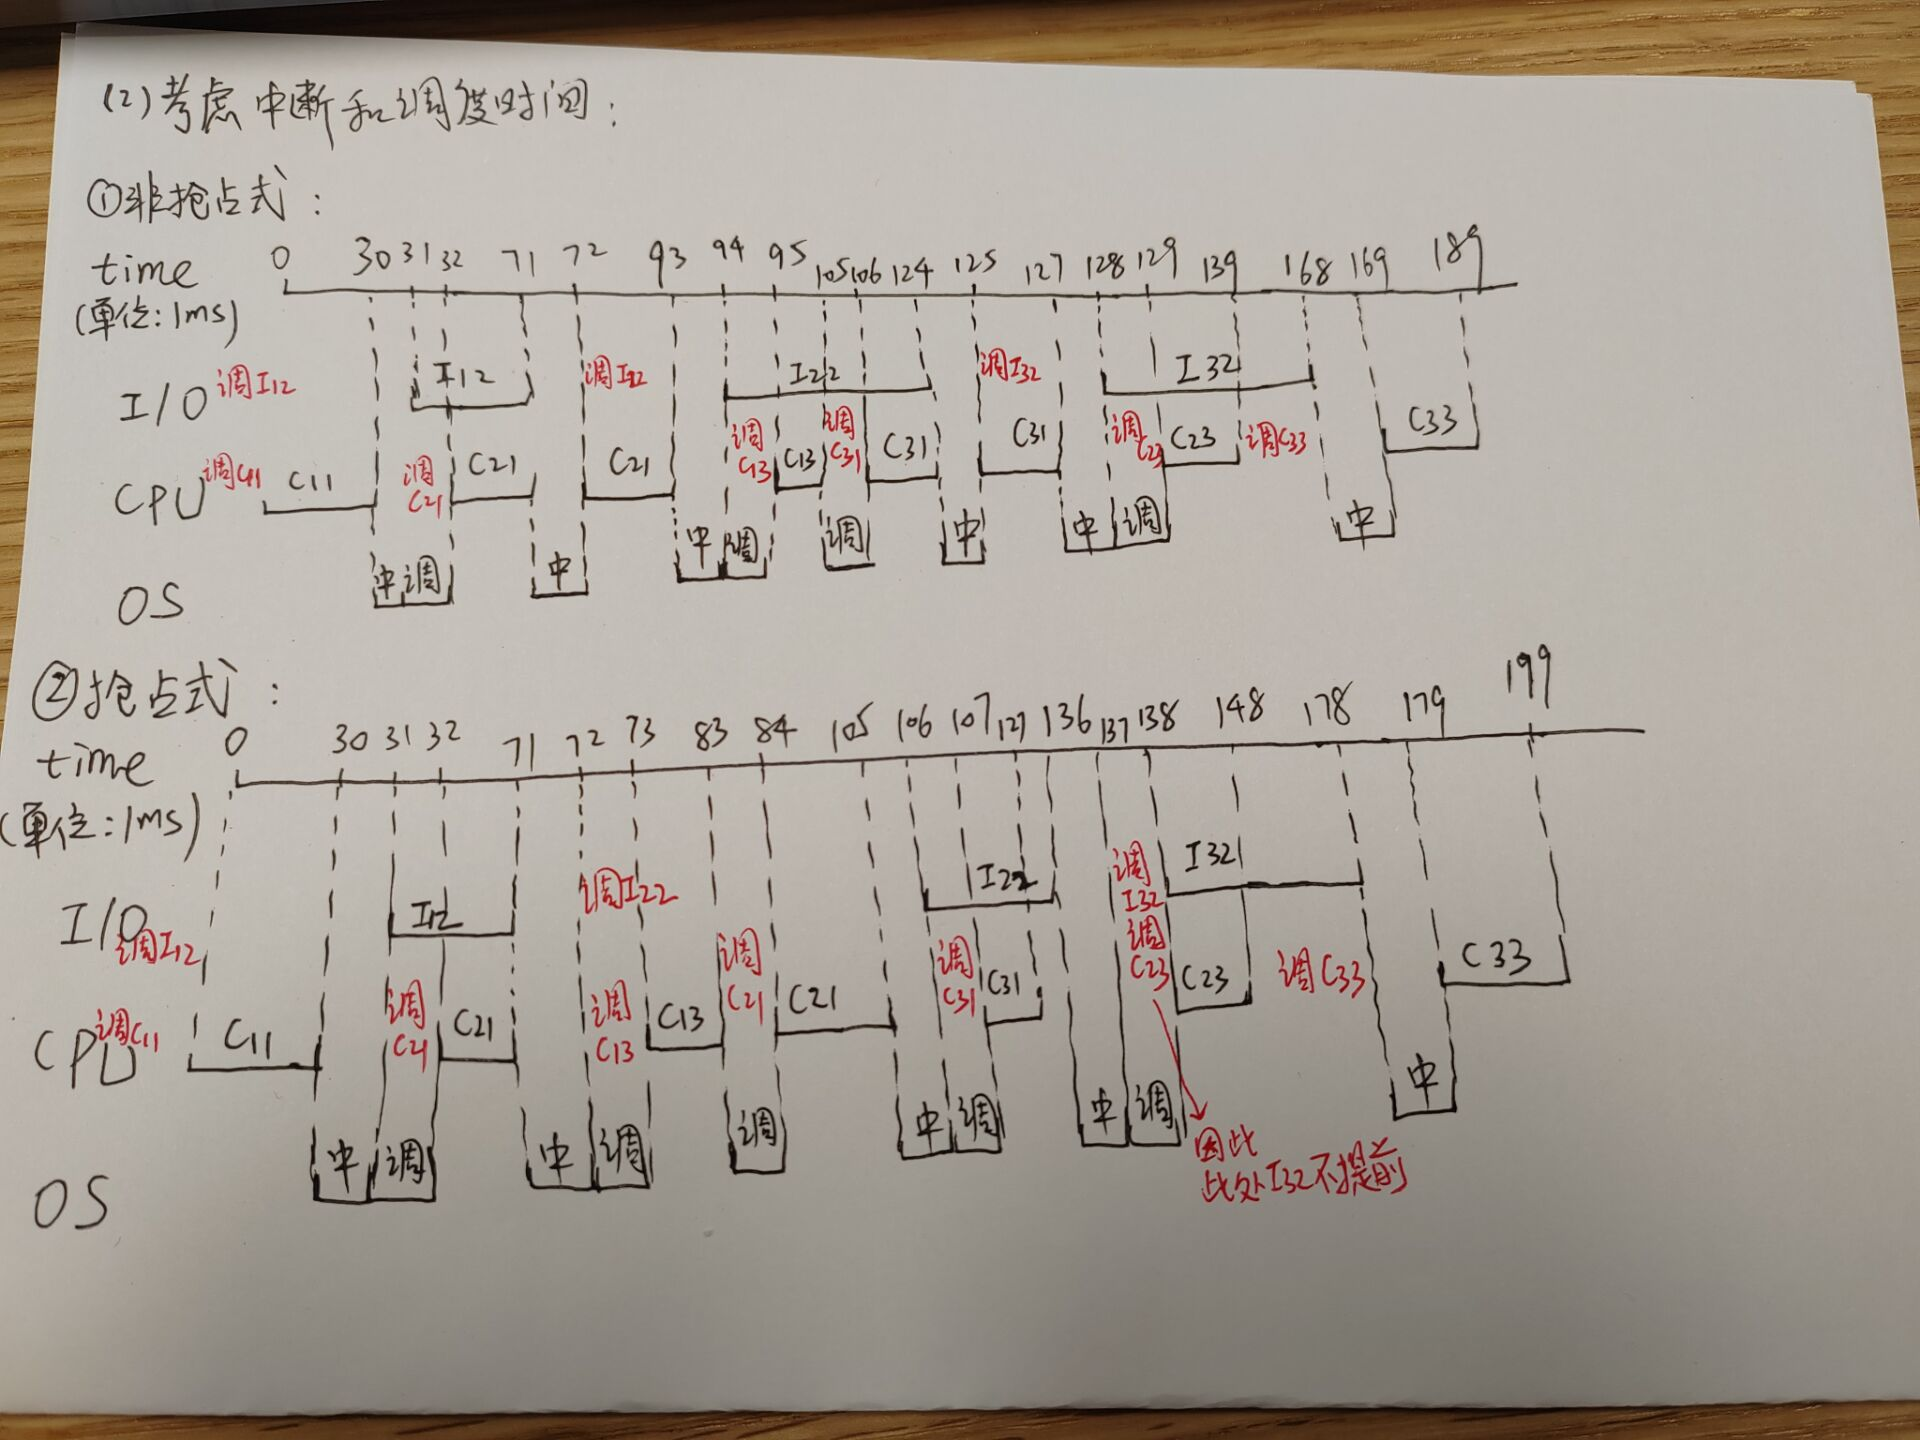
\includegraphics[width=0.7\linewidth]{C:/Users/86181/Desktop/figures/3}
	\caption{很丑的换行}
	\label{fig:3}
\end{figure}
	于是,我才用定义一个数据段保存打印的行号,每次打印后行号加1的方式来实现,解决了这个问题,代码相对简单,不在此展示。
	
	\subsubsection{优化makefile文件}
	此前,我的makefile需要两个指令才能运行结束,我做了修改,使得一个``make"指令就能直接跑起来,方便助教验收。

	\section{各种尝试、失败、debug过程}
	这部分是体现作业是自己做的的核心,这次作业,我遇到了非常非常多的问题
		
\begin{tikzpicture}[scale=0.2]
			% face
			\fill[red!20] (0,0) circle (2cm);
			
			% eyes
			\fill[white] (-0.6,0.5) circle (0.4cm);
			\fill[white] (0.6,0.5) circle (0.4cm);
			% left eye
			\fill[black] (-0.6,0.5) circle (0.2cm);
			% right eye
			\fill[black] (0.6,0.5) circle (0.2cm);
			
			% mouth
			\draw[line width=0.1cm] (-0.8,-1.3) .. controls (-0.4,-0.7) and (0.4,-0.7) .. (0.8,-1.3);	
		\end{tikzpicture},我解决了绝大部分,才得以得到上一部分展示的成功,接下来我将详细展示。
		
	\subsection{makefile失败!}
	在一开始makefile中我运行make的时候,始终报``Makefile:2: *** missing separator. Stop."我查找了文献得知这是缩进产生的问题。参考文献\href{https://blog.csdn.net/huamei13/article/details/106135901/}{\color{blue} Makefile:2: *** missing separator. Stop. 解决方法},我修改了我的缩进配置,但是仍然没有解决问题。偶然间我发现我的vscode里面的状态栏显示,我用的是空格进行缩进而不是tab,如下图所示。修改为采用tab缩进后立马解决了问题。
\begin{figure}[h!]
	\centering
	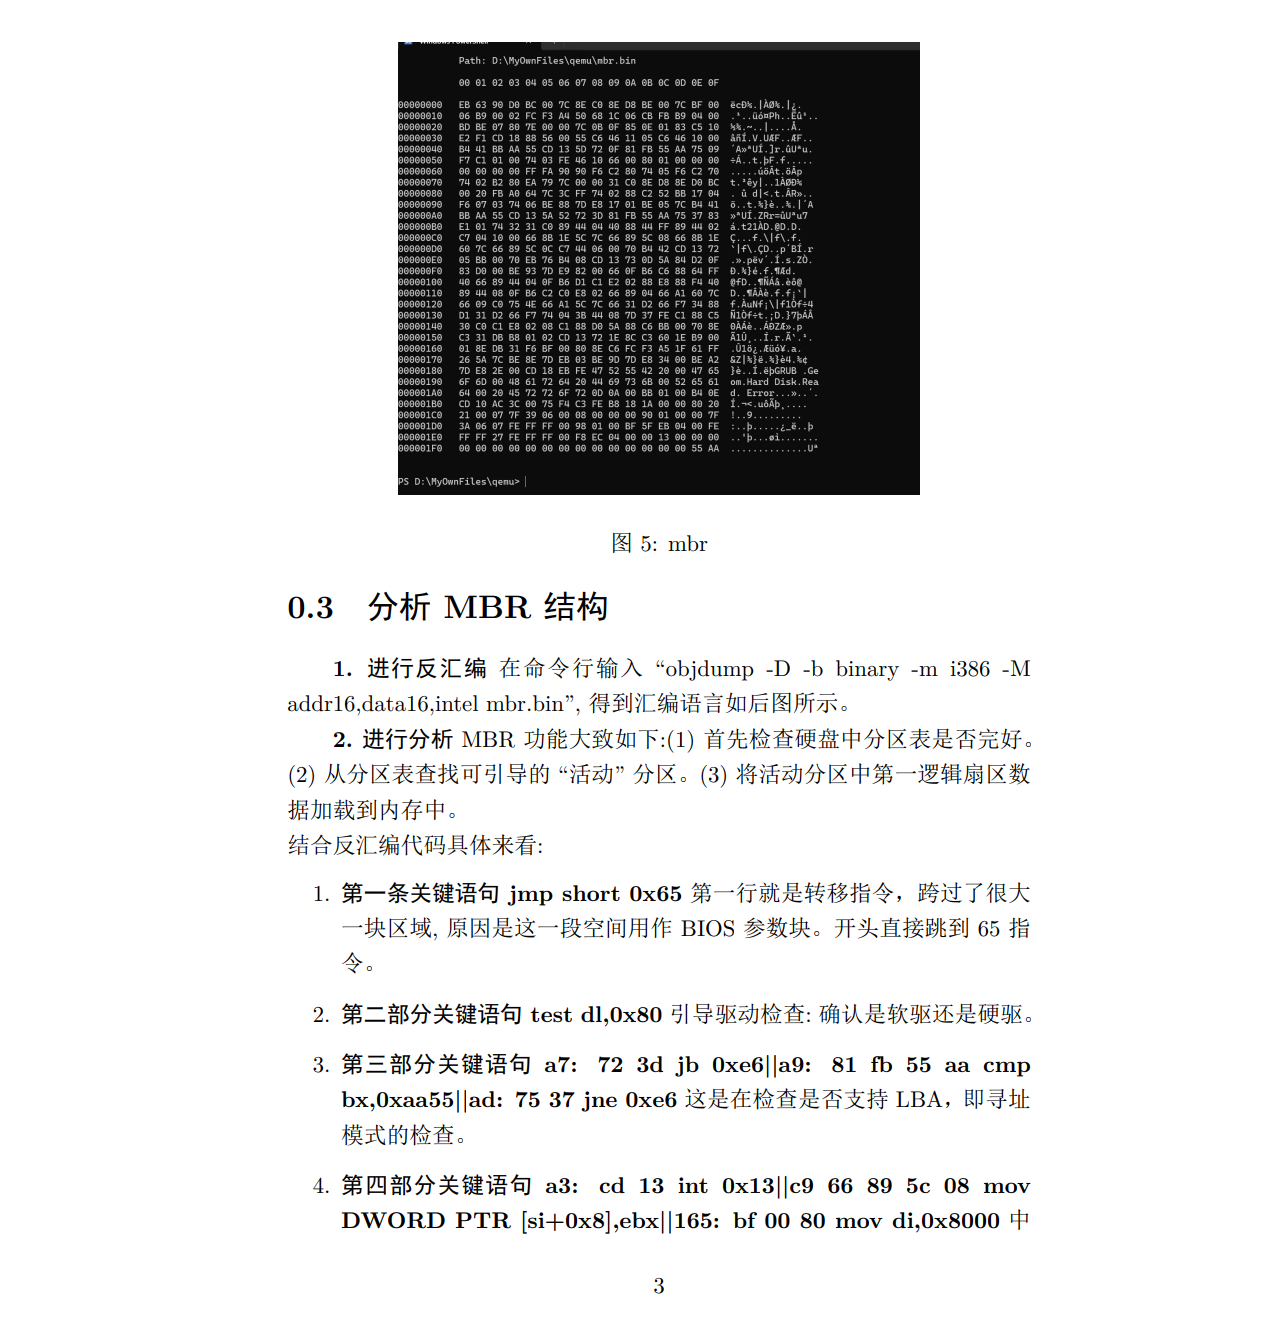
\includegraphics[width=0.7\linewidth]{C:/Users/86181/Desktop/figures/4}
	\label{fig:4}
\end{figure}
	
	
	\subsection{链接失败!}
	在编写链接文件的时候,我还遇到了``arm-linux-ld: warning: cannot find entry symbol \_start; defaulting to 00000000"的问题,这是由于我没用\_start来作为标签开始写代码,这很好解决。同时,链接失败还因为我代码运行的第一个函数不是main了,这通过objdump指令看了出来,所以我用了-e main指令告知程序入口是main。在其次,gcc编译的时候一定要用-m16,这样才能成功搞好。
	
	\subsection{关于打印换行的问题}
	我后来发现,我的代码打印到屏幕底端就会出现奇怪的显示,如下图所示。因此我又添加了一个计数器,统计一旦快打印到屏幕底端就清屏从头再打,这个代码相对简单,不在这里展示。最终解决了这个问题。\\\\\\
\begin{figure}[h!]
	\centering
	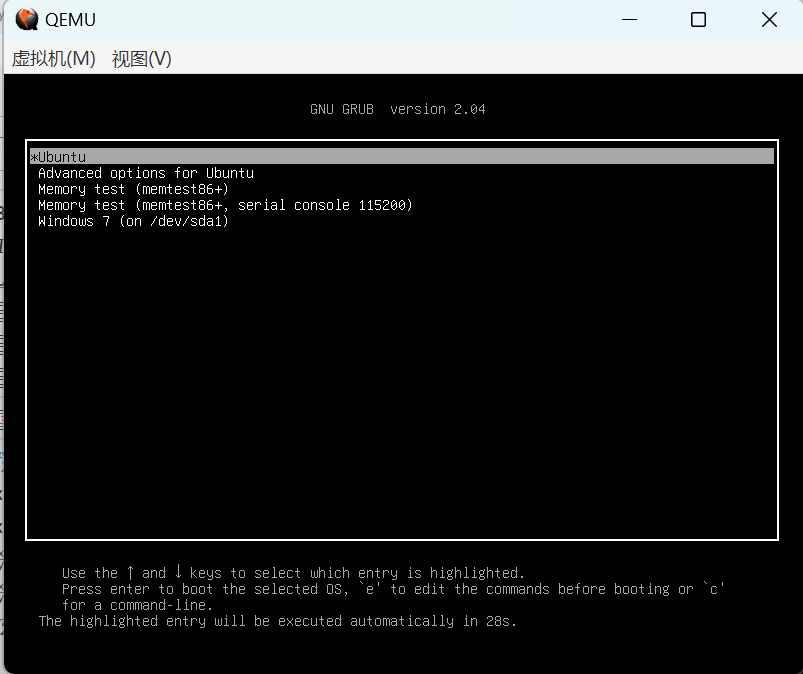
\includegraphics[width=0.7\linewidth]{C:/Users/86181/Desktop/figures/5}
	\caption{奇怪的打印}
	\label{fig:5}
\end{figure}

	\subsection{关于打印字符的问题}
	由于我的数据段一开始定义的刚刚好写到512字节结束,所以控制了打印的字符个数限制,导致我后来想再打印一个goodbye的时候出现了问题。我一开始以为是sleep实现错了,后来反应过来,将数据段在ld文件中的位置提前了一些,成功能够打印,发现还是sleep实现的有问题。
	
	\subsection{时钟中断停止了!}
	在某过程,我发现,我的代码只能打印两个hello和一个goodbye,表现如下图所示:
\begin{figure}[h!]
	\centering
	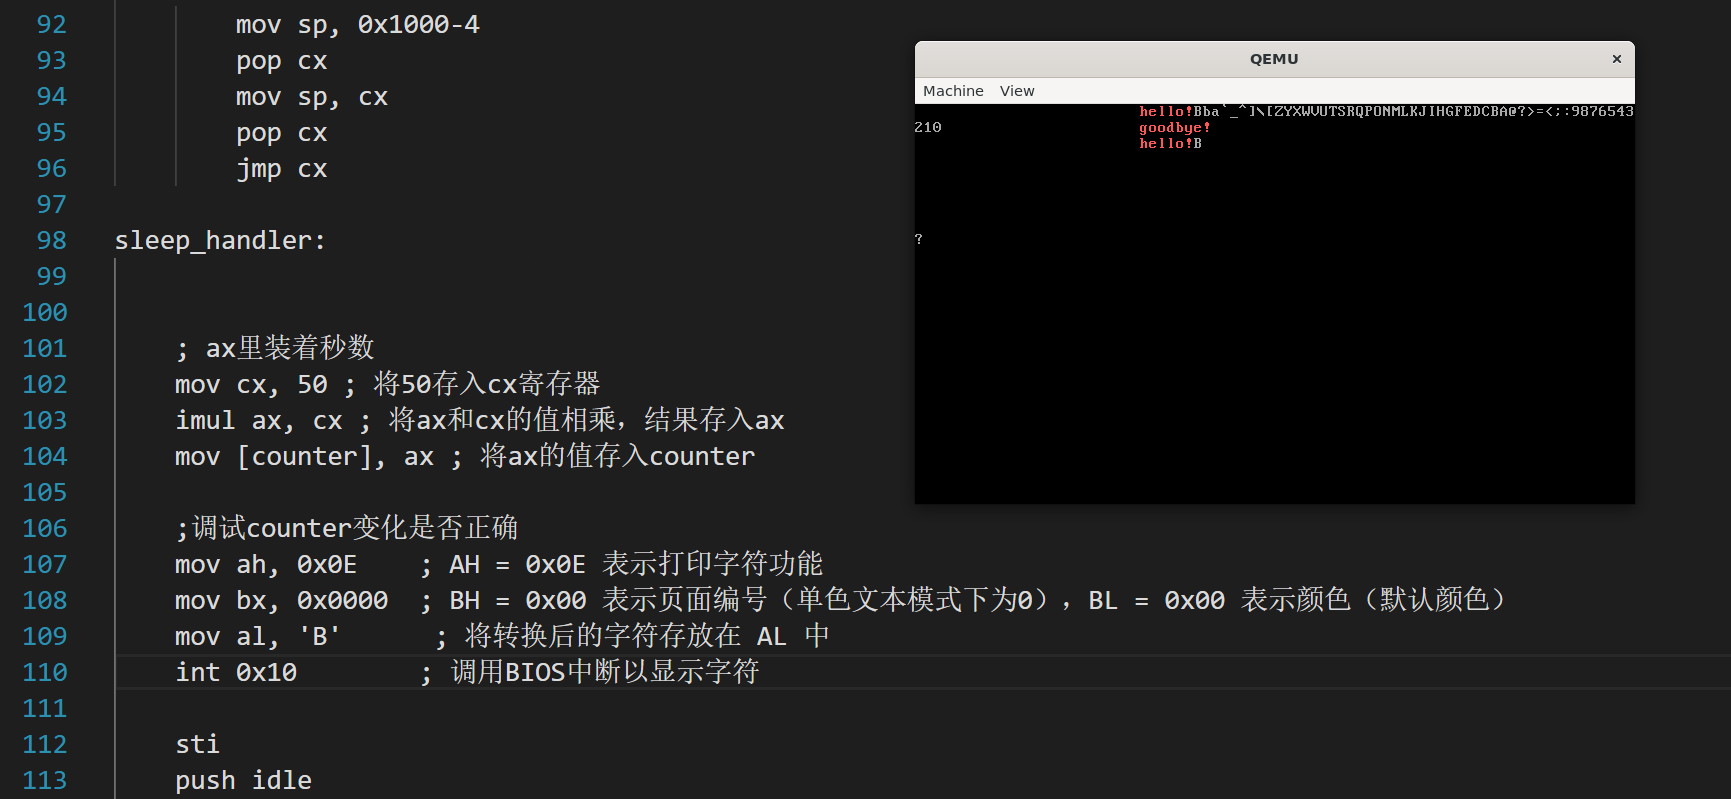
\includegraphics[width=0.7\linewidth]{C:/Users/86181/Desktop/figures/6}
	\caption{}
	\label{fig:6}
\end{figure}
	我编写了测试代码,将counter计数器的数值输出,以此来定位问题的位置。(此处我的实现是counter到0就应该打印一次)我将如下的代码放到时钟中断、sleep中断等各个位置测试:
\begin{lstlisting}[language=python,frame=shadowbox]
调试counter变化是否正确
mov ah, 0x0E    ; AH = 0x0E 表示打印字符功能
mov bx, 0x0000  ; 颜色
mov cx, [counter]
add cx, '0'     ; 将计数器的值转换为对应的 ASCII 字符
mov al, cl      ; 将转换后的字符存放在 AL 中
int 0x10        ; 调用BIOS中断以显示字符
\end{lstlisting}
	通过测试,我定位到问题在于时钟中断在第二次sleep进入内核的时候停止了!通过查阅资料,我得知这是由于我没有在是时钟中断iret之前告知时钟能继续产生新的中断,于是,我在对应位置加上如下代码,解决了问题:
\begin{lstlisting}[language=python,frame=shadowbox]
;告知中断完成,允许产生新中断
mov al,20h
out 20h,al
\end{lstlisting}
	
	\subsection{打印到16个左右hello就出bug!}
	在某过程,我发现,我的代码打印到16个hello/goodbye就会出问题,我检查代码,发现有个地方没有iret直接jmp到别的地方去了,这可能会导致栈乱掉或者其他的一些问题。我补上iret就重写了一下代码,解决了问题。
	
	\subsection{中断使用1ch不行8h可以}
	在此次作业中,我发现针对我的代码,时钟中断用1ch不行,用8h可以。这个问题我没有找到本质的答案,但是我猜测,可能是因为1ch是用户自定义中断,可以被屏蔽。以及1ch的iret指令回去的地方可能还需要做一些操作,才能让后续代码继续正常运行。
	
	\subsection{其他尝试:利用jmp切换进程}
	虽说这是不好的做法,但是我也为此花了不少时间。通过问助教,得知助教推荐使用反汇编语句找出app下一条语句位置进行跳转。我实现了一下,代码如下:
	\begin{lstlisting}[language=python,frame=shadowbox]
;api中代码
;不够好的实现,通过反汇编找回去的指令跳转
;与现代操作系统保护模式下内核回app不能用jmp不符合
not_that_good_sleep:
push ebp
mov ebp,esp
push eax
push ecx

mov eax,[ebp+8] ;获取参数

push 0x80ab ;通过反汇编得到,对应的int 0x81后的那条语句

mov ecx, esp
mov esp, 0x1000
push ecx
int 0x81
pop ecx
pop eax
pop ebp
retd
		
;kernel中跳转回main的代码	
mov sp, 0x1000-4
pop cx
mov sp, cx
pop cx
jmp cx
	\end{lstlisting}
	通过这种方法,也能达到作业的展示效果。同时,我还犯了一个错误,就是修改了main文件后忘了修改跳转地址,导致debug了一段时间。
	
	\subsection{其他问题}
	在安装wsl2以及处理linux和windows下make运行结果不同以及其他小的方面,还出过一些小问题,有过一些小尝试,不过均被我解决。同时,一开始并没有完全理解题意用iret方式实现进程切换,现在已经都改为iret。
	
	\section{总结与反思}
	\begin{itemize}
		\item 理论好理解不代表实验好做,实验需要非常多的细节,我反思我并没有在课上就完全理解老师的意思,导致我之前用jmp来切换进程,实际上这真的不合理,我后来意识到并且全部改为了iret
		\item STFW,RTFM 是计算机大类学生必备的素养,知识需要主动检索和学习
		\item 通过本次实验,我对一个简单的os内核有了更深的理解。我也明白了,像这种大的项目,一定需要有耐心一步一步的拆分、书写、调试。这两句话永远是对的:1.机器永远是对的 2.未经检验的代码永远是错的 ——蒋炎岩
	\end{itemize}

	\section{其它参考文献和致谢}
	除了正文给出的参考文献,我参考的文献还有:\\\\
	\href{https://blog.csdn.net/beyd3/article/details/120805234}{实现一个最简单的HelloOS内核}\\
	\href{https://blog.csdn.net/weixin_43903639/article/details/131341527}{ld链接脚本的编写}\\
	\href{https://blog.csdn.net/weixin_43216249/article/details/109827911}{汇编语言学习笔记 --数组和过程体的调用}\\
	\href{https://zhuanlan.zhihu.com/p/656259964}{嵌入式软件之链接脚本 .ld}\\
	\href{https://blog.csdn.net/qq_53004789/article/details/131354767}{makefile介绍}\\
	
	同时,衷心感谢与我一起研究讨论PA4的好朋友!
	
\begin{tikzpicture}[scale=0.2]
		% face
		\fill[blue!20] (0,0) circle (2cm);
		
		% eyes
		\fill[white] (-0.6,0.5) circle (0.4cm);
		\fill[white] (0.6,0.5) circle (0.4cm);
		% left eye
		\fill[black] (-0.6,0.5) circle (0.2cm);
		% right eye
		\fill[black] (0.6,0.5) circle (0.2cm);
		
		% mouth
		\draw[line width=0.1cm] (-0.8,-0.7) .. controls (-0.4,-1.3) and (0.4,-1.3) .. (0.8,-0.7);
	\end{tikzpicture}
	
\end{document}
